\chapter{Peking}

\begin{figure}[htbp]
\centering
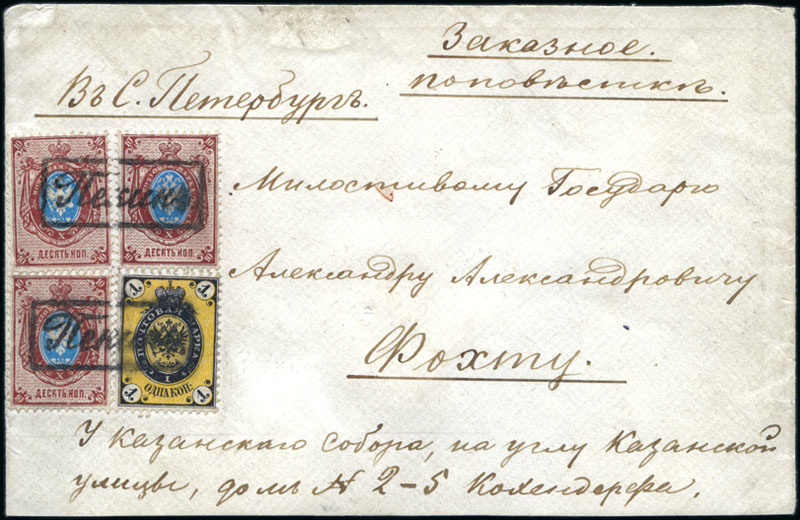
\includegraphics[width=.95\textwidth]{../russian-post-offices-in-china/10021.jpg}
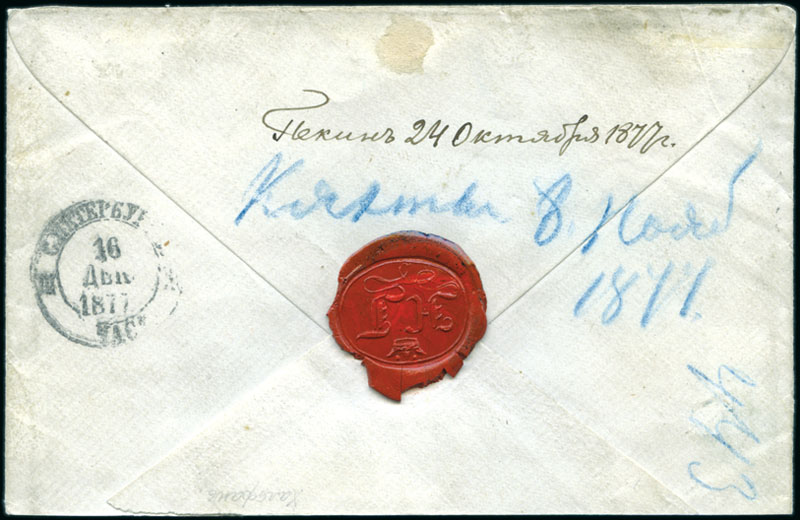
\includegraphics[width=.95\textwidth]{../russian-post-offices-in-china/10021-1.jpg}
\caption{
10021	POST OFFICES IN CHINA
PEKING: 1877 (Oct 24) Cover sent registered by notification to St. Petersburg 
with 1866 1k and three 1875 10k, paying double the 8k rate, 10k registration 
fee and 5k for certificate of posting, cancelled by boxed Peking hs, reverse 
with ms despatch and Kyakhta arrival and St. Petersburg receipt, cover slight 
trimmed at base.
This being the earliest known cover from the official Russian Post in Peking
Provenance: Ex Faberg\'e
\euro 70,000.00 
}  
\end{figure}

\begin{figure}[htbp]
\centering
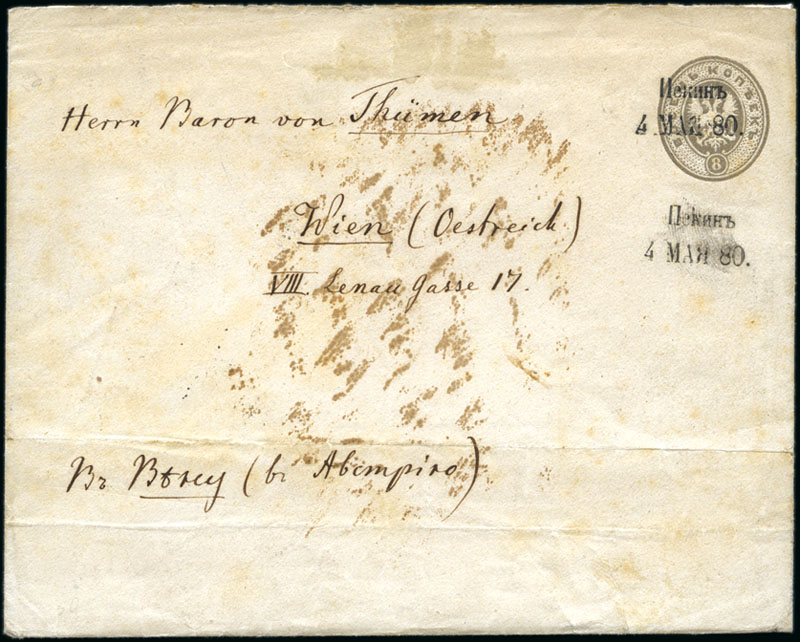
\includegraphics[width=.95\textwidth]{../russian-post-offices-in-china/10022.jpg}
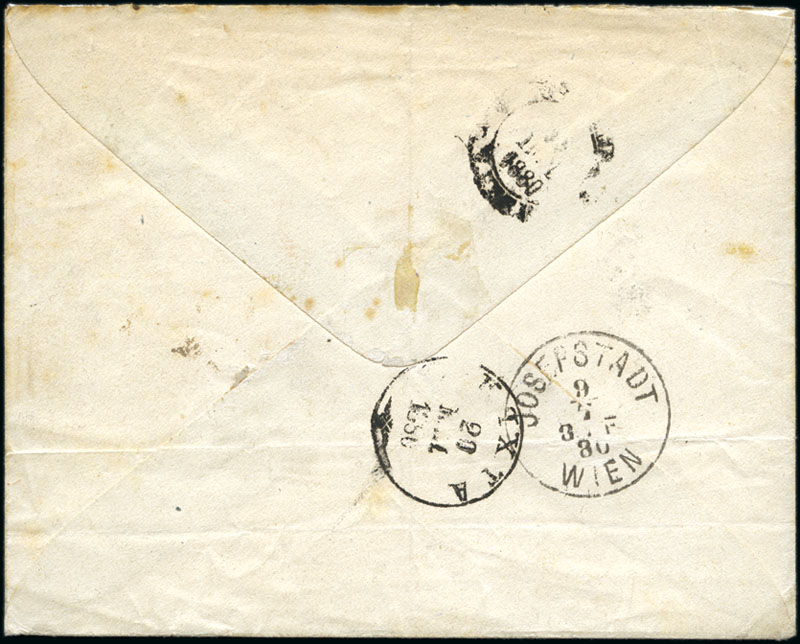
\includegraphics[width=.95\textwidth]{../russian-post-offices-in-china/10022-1.jpg}
\caption{
10022 PEKING: 1880 (May 4) 8k Postal stationery cover to Austria, 
cancelled by "PEKIN' / 4 MAY 1880" hs, with Kyakhta, Moscow and Vienna bs, 
taking 16 days to cross Mongolia and another 34 days to reach Moscow, 
one of only three known covers bearing this cancel
\euro 30,000.00 
}  
\end{figure}

\begin{figure}[htbp]
\centering
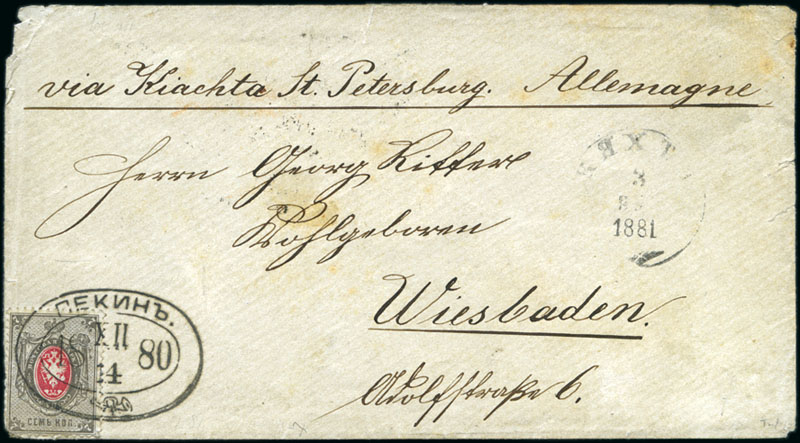
\includegraphics[width=.95\textwidth]{../russian-post-offices-in-china/10023.jpg}
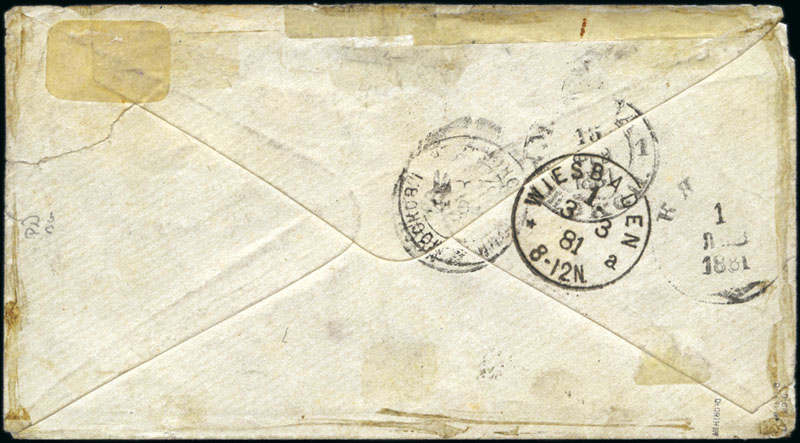
\includegraphics[width=.95\textwidth]{../russian-post-offices-in-china/10023-1.jpg}
\caption{
10023	ZoomPEKING: 1880 (Dec 14) Cover to Germany with 1879 7k tied by double 
oval Peking ds (Tchilinghirian type 3 variety, with month above day), with 
Kyakhta, Moscow and Wiesbaden bs.
Note: Illustrated in the British Journal of Russian Philately no.35 (1964) p.9
\euro 30,000.00 
}  
\end{figure}

                                                                                